\subsubsection{Задание 1.}

\begin{center}
   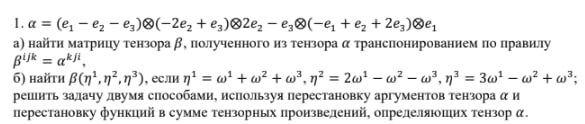
\includegraphics{assets/homework-3-task-1.jpg}
\end{center}

\textbf{Решение:}

a) Давайте найдем нашу $\sigma$. Она равна $(321)$. То есть, у нас такое транспонирование. Давайте тогда сначала надйем матрицу $\alpha \in T(0,3)$.
Если я не дурачок и умею считать,  то получается
$$\alpha  =\begin{pmatrix}[ccc|ccc|ccc]
    0 & 0 & 0 & 0 &-4 & 2 & 0 & 0 & 0 \\
    0 & 0 & 0 & 0 &4 & -2 & 0 & 0 & 0\\
    1 & -1 & -2 & 0 &4 & -2 & 0 & 0 & 0
\end{pmatrix}$$
Теперь транспонируем, у нас зафиксирован столбец:
$$\beta = \begin{pmatrix}[ccc|ccc|ccc]
     0 & 0 & 0 & 0 &0 & 0 & 1 & -1 & -2 \\
    0 & -4 & 2 & 0 &4 & -2 & 0 & 4 & -2\\
    0 & 0 & 0 & 0 &0 & 0 & 0 & 0 & 0
\end{pmatrix}$$
Все верно!

b) Найдем $\beta(\eta^1,\eta^2,\eta^3) = \beta(w^1 + w^2 + w^3, 2w^1-w^2-w^3,3w^1 -w^2 +w^3)$
Раскладываем эту штуку по линейности и получаем ответ. Но мне куда более нравится:
$$\beta(\eta^1,\eta^2,\eta^3) = \alpha(\eta^3,\eta^2,\eta^1)$$
Дальше мы просто подставляем в искомую и получаем $3\cdot 1\cdot2 - (1\cdot -5\cdot 1 ) = 11$

\subsubsection{Задание 2.}

\begin{center}
   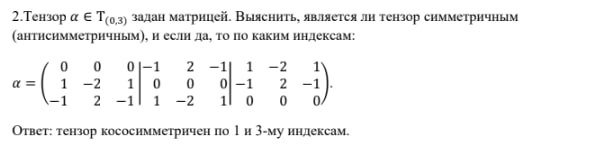
\includegraphics{assets/homework-3-task-2.jpg}
\end{center}

Я не знаю как это нормально делать, на глаз?

\subsubsection{Задание 3.}

\begin{center}
   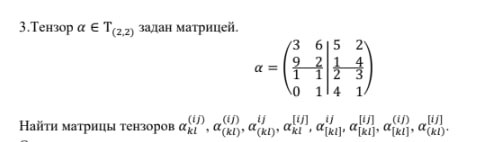
\includegraphics{assets/homework-3-task-3.jpg}
\end{center}

\textbf{Решение:}

Симметрирование - круглые скобки. Альтернирование - квадратные

1) $\alpha^{(ij)}_{kl} = \begin{pmatrix}
    3 & 15/2 & 5 & 3/2 \\
    15/2 & 2 & 3/2 & 4 \\
    1 & 1/2 & 2 & 7/2 \\
    1/2 & 1 & 7/2 & 1
\end{pmatrix}$

В данном случае слой и сечение зафиксированы, так что чилл море песок, нам всего лишь надо просимметрировать квадратные матрички.

2)  В данном случае порядок симметрирования не имеет значения.

$\alpha^{(ij)}_{(kl)} = \begin{pmatrix}
    3 & 15/2 & 3 & 1 \\
    15/2 & 2 & 1 & 5/2 \\
    3 & 1 & 2 & 7/2 \\
    1 & 5/2 & 7/2 & 1
\end{pmatrix}$

3) $\alpha^{ij}_{(kl)} =\begin{pmatrix}
    3 & 6 & 3 & 3/2\\
    9 & 2 & 1/2 & 5/2 \\
    3 & 3/2 & 2 & 3 \\
    1/2 & 5/2 & 4 & 1
\end{pmatrix}$

4) $\alpha^{[ij]}_{kl} = \begin{pmatrix}
    0 & -3/2 & 0 & 1/2 \\
    3/2 & 0 & -1/2 & 0 \\
    0 & 1/2 & 0 & -1/2\\
    -1/2 & 0 & 1/2 & 0
\end{pmatrix}$

В данном примере у нас происходит альтернирование в каждой части

5) $\alpha^{ij}_{[kl]} = \begin{pmatrix}
    0 & 0 & 2 & 1/2\\
    0 & 0 &1/2 & 3/2 \\
    -2 & -1/2 & 0 & 0 \\
    -1/2 & -3/2 & 0 & 0
\end{pmatrix}$

6) $\alpha^{[ij]}_{[kl]} = \begin{pmatrix}
    0 & 0 & 0 & 0\\
    0 & 0 &0 & 0 \\
    0 & 0 & 0 & 0 \\
    0 & 0 & 0 & 0
\end{pmatrix}$

7)$\alpha^{(ij)}_{[kl]} = \begin{pmatrix}
    0 & 0 & 2 & 1/2\\
    0 & 0 &1/2 & 3/2 \\
    -2 & -1/2 & 0 & 0 \\
    -1/2 & -3/2 & 0 & 0
\end{pmatrix}$

8) $\alpha^{[ij]}_{(kl)} = \begin{pmatrix}
    0 & -3/2 & 0 & 1/2 \\
    3/2 & 0 & -1/2 & 0 \\
    0 & 1/2 & 0 & -1/2\\
    -1/2 & 0 & 1/2 & 0
\end{pmatrix}$

\subsubsection{Задание 4.}

\begin{center}
   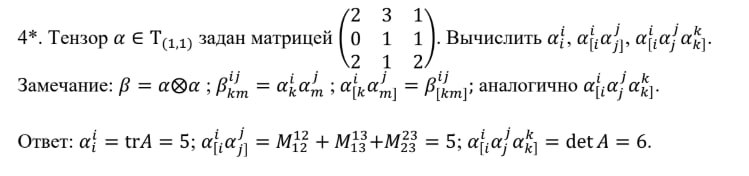
\includegraphics[width = 14cm]{assets/homework-3-task-4.jpg}
\end{center}

\textbf{Решение.}

Ну в первом случае это просто след матрицы.

$\beta^{ij}_{kl} = \alpha^{i}_{k}\otimes \alpha^{j}_k$

Заметим, что альтернируя по нижним индексам, мы получим, что на совпадающих $i,j$ стоят нули, откуда нам надо сложить только челиков, на несовпадающих. При этом не забыв про альтернировать. Откуда уже вроде получается нужное

